\chapter{An Empirical Study on SQL Semantic Bugs in the Wild}
\label{chapter:semantic_bugs_study}

\section{Research methodology}
\label{section:research_methodology}

In this section we will present the research questions that this paper tries to answer. Furthermore, we also provide some more details regarding the datasets used in this research.

\begin{mdframed}
\noindent \textbf{RQ1:} \emph{What is the prevalence of semantic bugs in SQL queries?}
\end{mdframed}

With this research question, the aim is to investigate which are the most prevalent semantic bugs that appear in SQL queries. In order to analyse this, one of the most important aspects is being able to collect queries used in real world systems. For this, two datasets are used, one containing queries extracted from StackOverflow posts, and another dataset provided by \citet{P011} in their study on search-based test data generation for SQL queries. Both of these contain queries used in various open source projects and should provide a clear answer as to how often semantic bugs appear in SQL queries. To answer the question, we will run the rule-based static analysis tool designed for this project on all the collected queries and report on the total number of issues detected for each semantic bug. Furthermore, we also determine the median prevalence for each semantic bug as the ratio between the total number of queries having the semantic bug and the total number of collected queries in the dataset.

\begin{mdframed}
\noindent \textbf{RQ2:} \emph{What are the co-occurrences of semantic bugs in SQL queries?}
\end{mdframed}

The aim of this research question is to understand whether certain semantic bugs might tend to appear in pairs. It is valuable to know whether this is the case since if certain errors are detected in a query, then further attention can be paid to bugs that might co-occur. For answering this question, we use the results obtained for RQ1 from running the tool on all the collected queries, and then build a co-occurrence matrix for the semantic bugs. Furthermore, we also use the techniques described by \citet{P012} in order to compute the Jaccard index for normalizing co-occurrence data and present this in the form of a heat map. The Jaccard index is defined as the ratio between the number of times two bugs co-occur and the number of times for which at least one bug is observed to be present.

\begin{mdframed}
\noindent \textbf{RQ3:} \emph{What is the correlation between the complexity of a query and the number of semantic bugs it has?}
\end{mdframed}

Another interesting insight is knowing whether the complexity of a query has any correlation with the number of semantic bugs it has. By having this knowledge, whenever a query is detected as being too complex, this can already signal that potential semantic bugs might be present in the formulation of the query. In order to answer this question, we define and compute the complexity of a query as the total number of predicates, joins, subqueries, functions and columns it contains.

For analysing the correlation between the complexity of the query and the number of semantic bugs it has we will provide a box plot, which is the preferred visualization technique when dealing with both numerical and categorical data such as the one in our case, as described by \citet{P992} in their book on data visualization techniques. Furthermore we also provide the distribution for the query complexity scores. The data used in these visualizations will include our entire collection of SQL queries, from both the StackOverflow and the EvoSQL datasets.

Finally, we perform the one-way analysis of variance (ANOVA) test as described by \citet{P991} in order to determine whether or not there is a statistically significant difference between the means of our groups, which are given by the number of semantic bugs per query.

\section{Data collection}
\label{section:data_collection}
In this section we describe the approach used for building a large dataset of SQL queries collected from StackOverflow posts. StackOverflow is the main website where developers can ask questions and discuss various computer programming related issues which makes it one of the largest knowledge bases in this field. Apart from the 170,000 queries collected from StackOverflow, we also used for our study the dataset provided by \citet{P011} in their paper, which contains an additional 19,159 SQL queries extracted from various open source projects on GitHub.

The technique we used for extracting SQL queries from StackOverflow posts focused on retrieving the code block sections from each post and parsing these for finding valid SQL statements. For this, using an API for accessing the available StackOverflow data was preferred over other techniques such as web crawling since using an API is less intrusive for the StackOverflow platform. Google’s BigQuery public datasets now also include StackOverflow data, however these are not always up to date and further analysis showed these datasets are also not complete. In the end, for this paper, it was decided to use the Stack Exchange API\footnote{\url{https://api.stackexchange.com/}} which provides an interface for retrieving posts data from StackOverflow. Our query extraction tool only looks at SQL tagged questions, since these are the most likely to contain the queries we are interested in. Furthermore, before starting to process the posts, we filtered them on the number of votes they had, and sorted them in descending order, such that the more relevant and higher quality posts were processed first. In total, there are roughly 11,000 pages with SQL tagged questions on StackOverflow. For our study, we processed and extracted the queries from the top ranked 2000 pages. Our tool is capable of processing all pages, however we considered that enough queries were extracted to build a good dataset on which we could test our rule-based static analysis tool. Further studies could use the tool we developed in order to obtain an even larger dataset of queries should this be needed.

The Stack Exchange API offers functionality for creating a custom filter which is then included in the request providing fine control over the returned data. For our project, all metadata associated with a post was collected since the goal was building a complete dataset which might later be used for other research as well. Furthermore, it is important to point out that a distinction should be made between a question post and an answer post. A question post can have multiple answers associated with it and should also have at most one accepted answer. All posts, questions and answers, are created by one user, and have a score associated with them which indicates the number of upvotes a question or an answer has received. The intuition behind the score value for questions is that the higher the number, the more developers found that particular question useful, whereas for answers the higher the score the better the answer.

The collected data was organized in a MySQL database with four important schemas: owners, questions, answers and queries. In the owners table, the data about the user who created the post is stored together with any other metadata associated with the user. In the questions table, the data for the questions posts is stored and similarly in the answers table the data for all other posts is stored. Finally, in the queries table all extracted queries are saved together with an identifier which links the query to the post from which it was extracted. Since StackOverflow has no way of enforcing SQL syntax to be written in code block sections, this means that users are free to input any type of text inside the code blocks. Because of this, a special algorithm has to be used for extracting only the SQL statements from these sections.

Our approach for query extraction can be seen as an island parsing technique, similar to the solution proposed in \citet{P028}, where typically some recognizable structures are being parsed with detailed rules describing the constructs of interest, in our case the SQL keywords (the islands), and the remaining parts (the water), which in our case represent the overall query statement, are captured with other more generic rules. The algorithm used for extracting the queries from the code block section starts by first looking at every line and detecting whether it starts with a valid SQL keyword. If not, a number of additional checks are carried out in order to determine whether the line is part of an enumeration which was split on multiple rows. If this is still not the case, then the line is eliminated from the code block. After all lines from a code block section are parsed, all of them are collected into a single query. In case users input multiple SQL queries the algorithm also detects this by looking for the special semicolon character which indicates the end of an SQL statement. Another approach was also considered for the query extraction algorithm, which constructed the abstract syntax tree (AST) for each of the code blocks, however since these blocks might also contain non-SQL syntax as well, it was observed that more queries were extracted with the previous approach. Furthermore, another potential method could have been using a tool such as GitHub linguist\footnote{\url{https://github.com/github/linguist}} for automatically detecting the type of code present in the snippets and continue with further processing if SQL would have been detected. However, we did not explore this approach, but it might be something interesting to investigate in future studies on mining data from StackOverflow. Finally, all extracted queries are saved in the MySQL database and can later be processed by other tools such as SQL parsers like JSQLParser for determining whether the syntax of the query is indeed valid. We provide some descriptive statistics for the collected dataset in Table \ref{table:stackoverflow_stats}. The tool which extracts the queries is also made available on the GitHub page for our project at the following link: \url{https://github.com/cldme/SQLBugFinder/tree/main/queries_stack_exchange}

\begin{table}[ht]
\centering
\begin{tabular}{@{}lr@{}}
\toprule
\textbf{Statistic}                         & \textbf{Measurement} \\ \midrule
Total queries                              & 394,477         \\
Valid syntax                               & 172,232         \\
Invalid syntax                             & 22,2245         \\
Average response time for SQL questions    & 14m 54s        \\
Queries with semantic bugs                 & 28,386          \\
Queries with 1 semantic bug                & 24,229          \\
Queries with 2 semantic bugs               & 3572           \\
Queries with 3 semantic bugs               & 551            \\
Queries with 4 semantic bugs               & 32             \\
Queries with \textgreater{}5 semantic bugs & 2              \\ \bottomrule
\end{tabular}
\caption{General statistics for the StackOverflow dataset}
\label{table:stackoverflow_stats}
\end{table}

\section{Results}
\label{section:results}
In the following sections we discuss the results for each of the research questions and present our findings.

\subsection{RQ1: What is the prevalence of semantic bugs in SQL queries?}

We ran the rule-based static analysis tool containing 25 rules for detecting various SQL semantic bugs, as explained in Section \ref{section:detection_strategies}, on all collected queries. We observe that out of all 191,994 queries, a total of 36,818 queries which contain at least one semantic bug were identified, meaning that 19.17\% of queries contained some semantic problem in their formulation. Again, this shows the need for providing semantic bug detection tools for developers in order to improve the overall quality of SQL queries used in real world applications.

In Figure \ref{fig:prevalence} we show the prevalence of the detected semantic bugs in our StackOverflow dataset. Out of all these bugs, the most frequent one is the missing join predicates semantic bug (\sql{E019}), with a median prevalence of 5.98\%. The second most frequent semantic bug is the constant output column (\sql{E002}), which has a median prevalence of 3.62\% closely followed by the unnecessary count argument bug (\sql{E012}) with a median prevalence of 3.35\%. We did not detect any semantic bugs related to the use of identical tuple variables (\sql{E005}) in our collected dataset. For most of the other rules, the median prevalence was below 0.5\%, which means that out of 200 queries, one will be affected by a semantic bug.
We further analysed the rule for detecting missing join predicates by selecting 20 random queries for which this error was reported and manually checking the results of our tool. In all cases, we concluded that there were no false positive warnings and all errors were detected correctly. The same manual analysis was also conducted for all the other rules and we included the results in Appendix \ref{appendix:tool_validation}.

Other previous studies such as those conducted by \citet{P001} and \citet{P003} also concluded that the missing join predicates semantic bug is indeed frequent in SQL queries. One noticeable difference between previous study and our work comes from the datasets used. Most of the past work is based on queries collected from SQL courses, which means that queries are written by students on exams and other homework material. In our dataset, we used queries from various open source projects, hence the slightly lower median prevalence. Interestingly enough, \citet{P003} reports on 3.6\% prevalence for the constant output column semantic bug, again on a dataset of queries written by students on various exams, which is very close to the median prevalence we found in our study for the StackOverflow dataset, of 3.62\%.

In Figure \ref{fig:prevalence_evosql} we show the prevalence of the detected semantic bugs in the EvoSQL\footnote{\url{https://www.zenodo.org/record/1166023}} dataset. This dataset only contains SQL \sql{SELECT} queries found in three open source projects tracked on GitHub. Upon further manual inspection, it was observed that most of the queries suffered from the implicit columns SQL semantic code smell as described in the works of both \citet{P010} and \citet{P998}. In our implementation, this SQL semantic error corresponds to the constant output column bug (\sql{E002}), and as it can be observed from the results of our tool, this bug is indeed the most frequent one in the EvoSQL dataset with a median prevalence of 43.23\%. For all other semantic bugs, our tool detected a median prevalence of less than 0.4\% for this dataset.

\begin{mdframed}[default]
\noindent \textbf{RQ1 summary:} Out of all the collected queries, 19.17\% contained at least one semantic bug. The most common bugs are the missing join predicates (\sql{E019}) followed by the constant output column (\sql{E002}) and unnecessary count argument (\sql{E012}) bugs.
\end{mdframed}

\begin{figure}[ht]
    \centering
    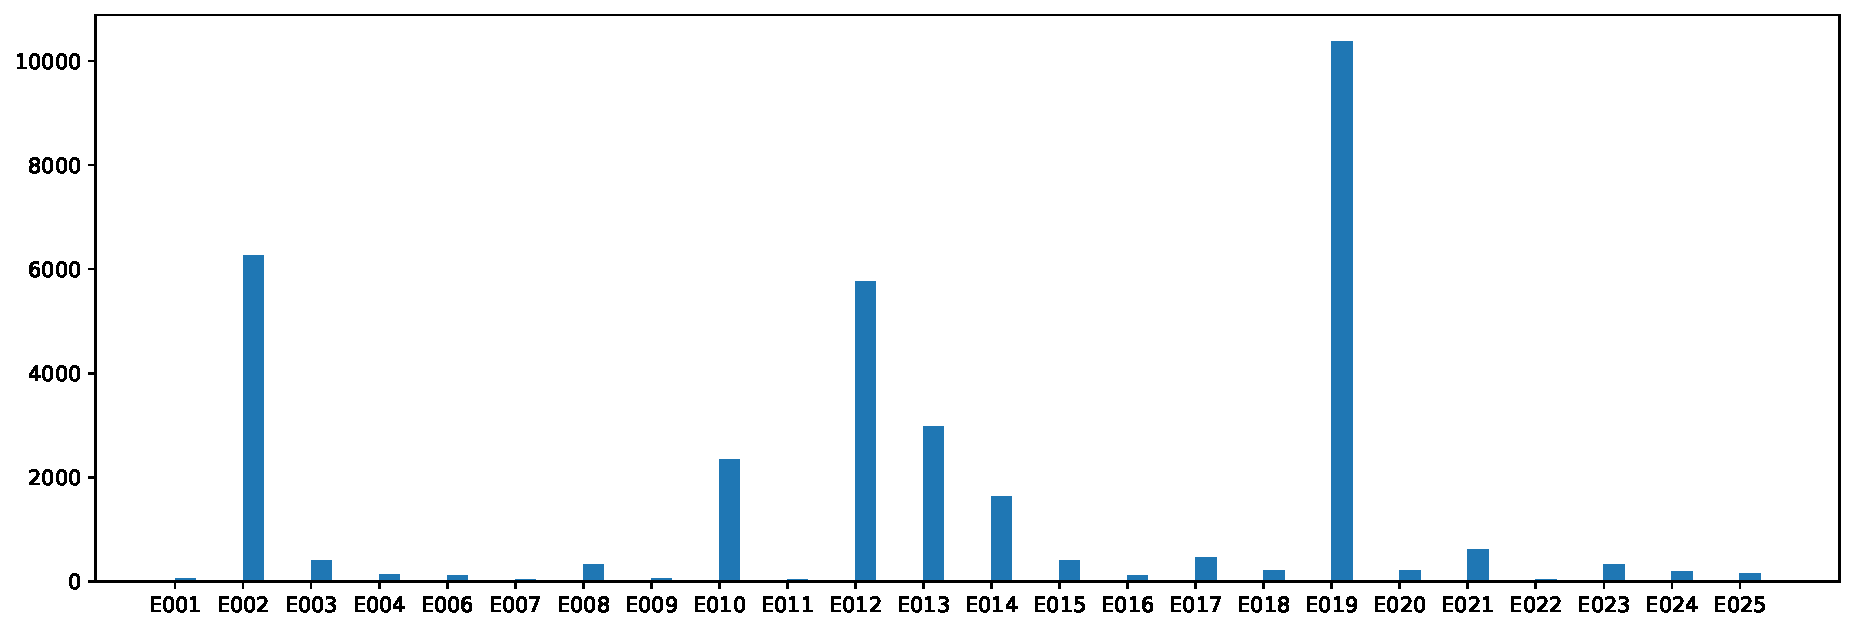
\includegraphics[width=1\textwidth]{img/prevalence.pdf}
    \caption{Prevalence of SQL semantic bugs for the StackOverflow dataset}
    \label{fig:prevalence}
\end{figure}

\begin{figure}[ht]
    \centering
    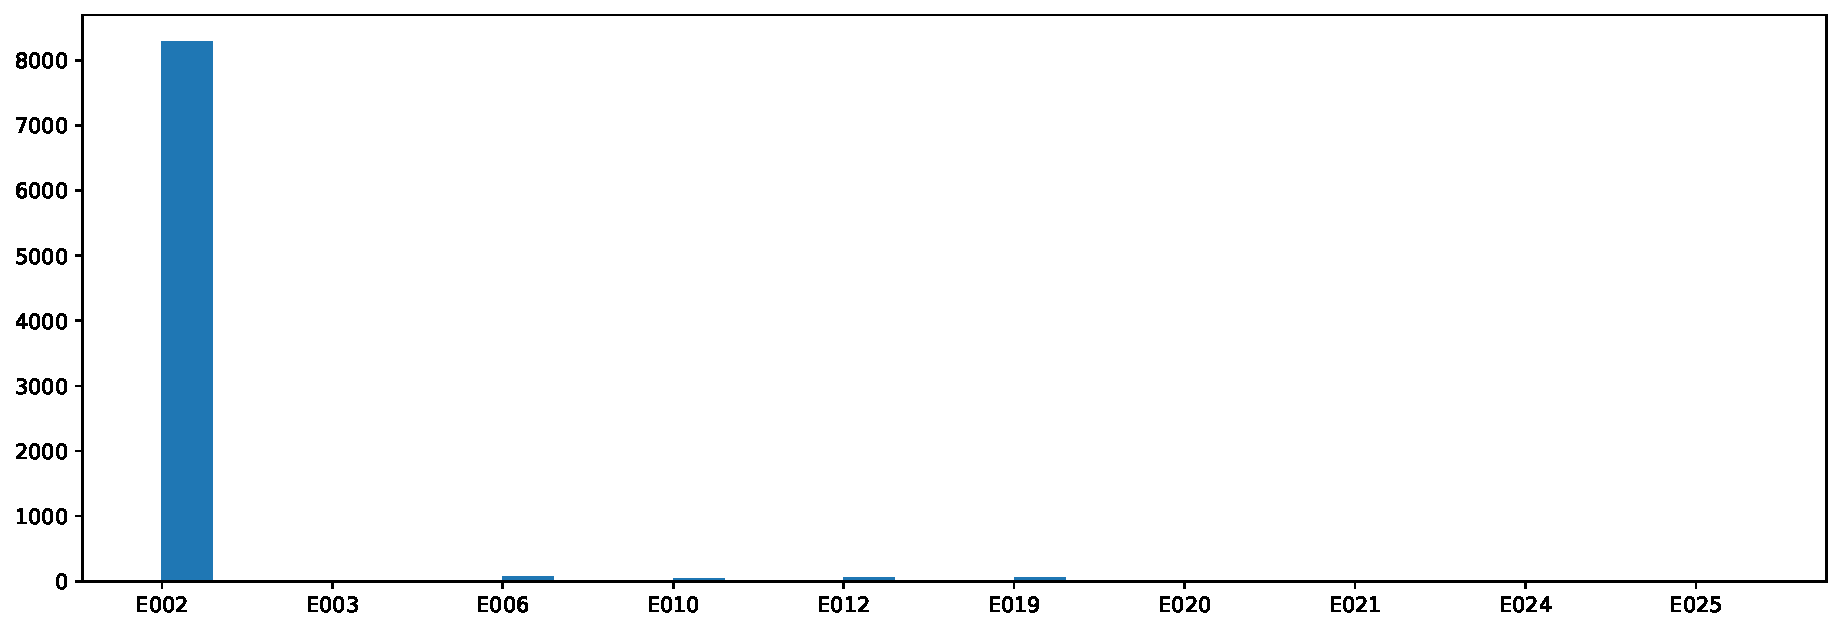
\includegraphics[width=1\textwidth]{img/prevalence_evosql.pdf}
    \caption{Prevalence of SQL semantic bugs for the EvoSQL dataset}
    \label{fig:prevalence_evosql}
\end{figure}

\subsection{RQ2: What are the co-occurrences of semantic bugs in SQL queries?}

In Figure \ref{fig:matrix} we show the co-occurrence matrix for our entire dataset, where each entry in the matrix represents the Jaccard similarity coefficient as described by \citet{P012} (empty cells have value zero). From this, we observe that most of the similarity values are rather low, however there is a 20\% similarity between bugs \sql{E012} and \sql{E013}, as well as a 15\% similarity between bugs \sql{E012} and \sql{E019}, followed by a 15\% similarity for bugs \sql{E002} and \sql{E019}. The Jaccard index is a measure of similarity between two sets of data, ranging from 0\% to 100\%, which means the higher the percentage, the more similar the two sets are to one another. In our case, for two bugs say A and B, if these have a 30\% similarity measure, this means that if bug A is detected in one query, then there is a 30\% probability that bug B is also present in this query.

This type of insight can be useful in designing future detection tools as well as prediction systems that could be integrated within IDEs in order to alert developers regarding certain bugs that their queries might contain given bugs which have already been detected. Further manual inspection for the queries where both the unnecessary count argument bug (\sql{E012}) as well as the unnecessary group by attribute error (\sql{E013}) both occur reveals that indeed these two types of semantic bugs are more likely to co-occur since usually the \sql{GROUP BY} clause is used with the intention of aggregating some data in the \sql{SELECT} clause.

Another interesting finding is that the missing join predicate bug (\sql{E019}) is the most likely one to co-occur with other types of bugs. More concretely, there is a 15\% similarity between queries containing bug \sql{E019} and either bug \sql{E002} or \sql{E012} and a 10\% similarity between queries containing bug \sql{E019} and either bug \sql{E013} or \sql{E015}. This also matches with the findings from \textbf{RQ1} which showed that bug \sql{E019} is the most prevalent one in our entire dataset, and as a result it co-occurs with 4 other different error types. 

\begin{mdframed}[default]
\noindent \textbf{RQ2 summary:} The co-occurrence of semantic bugs in SQL queries for our entire dataset is rather low, indicating that queries rarely contain more than one semantic bug. The highest similarity between two bugs is 20\%, for the unnecessary count argument (\sql{E012}) and unnecessary group by attribute (\sql{E013}).
\end{mdframed}

\begin{figure}[ht]
    \centering
    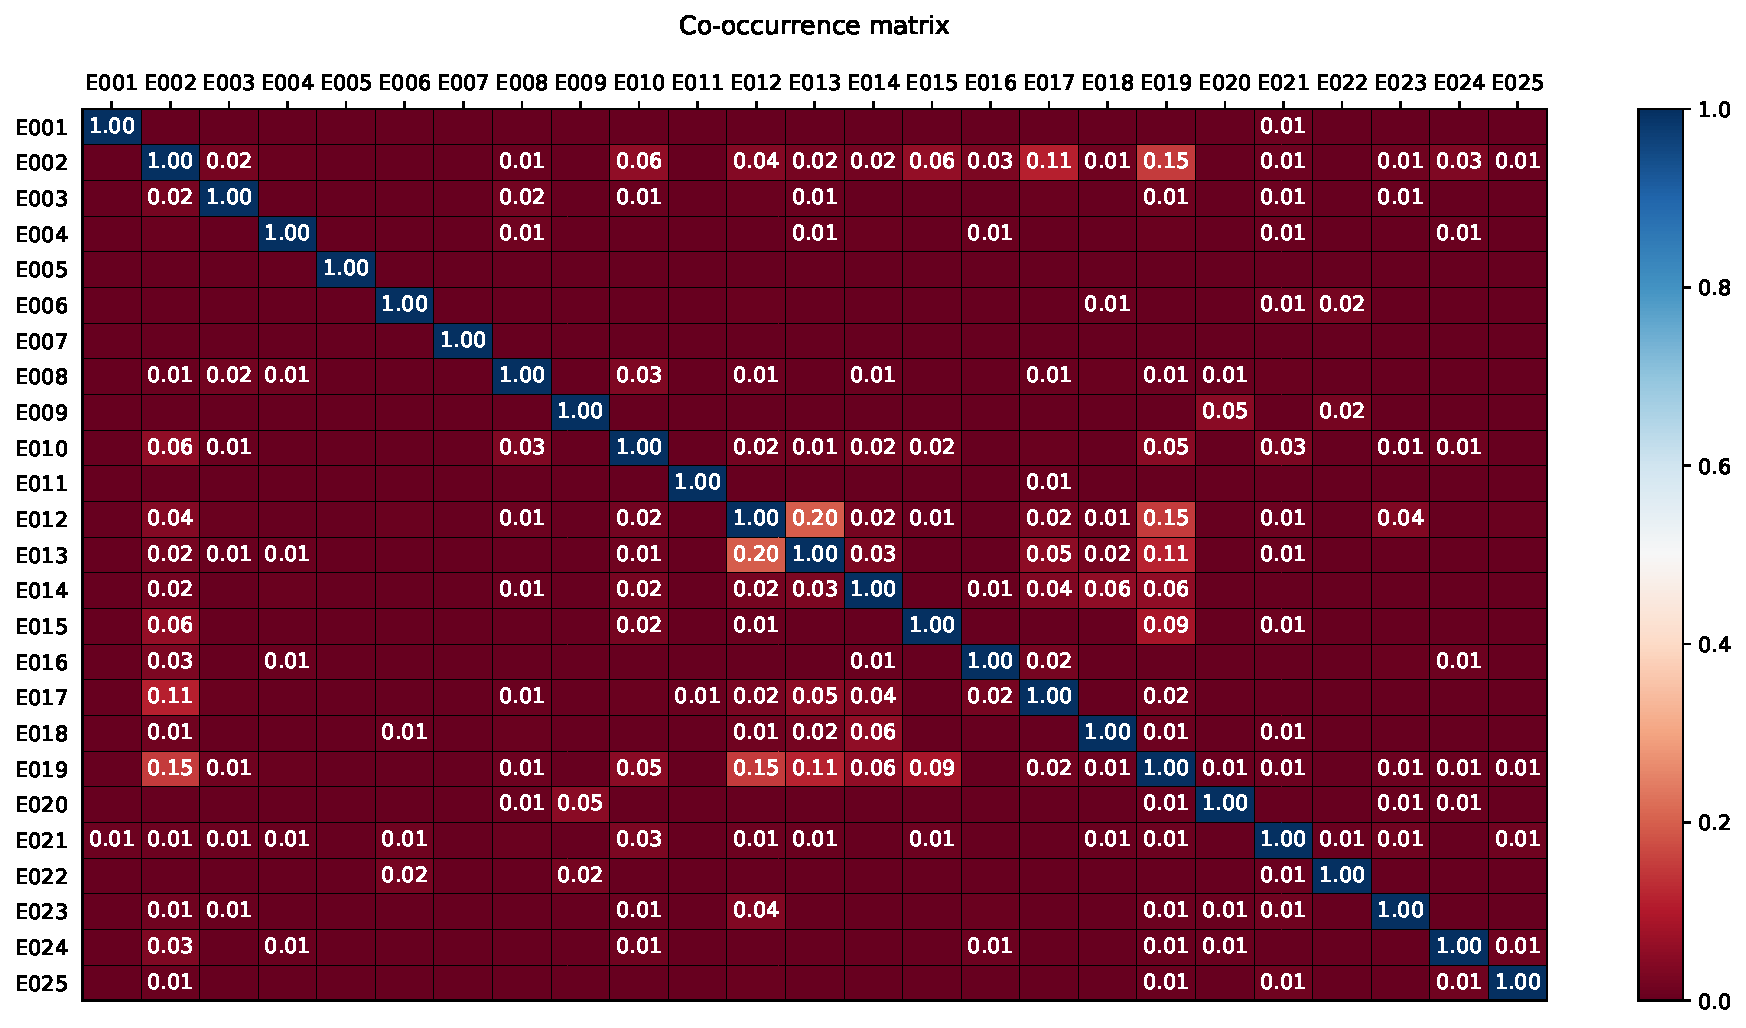
\includegraphics[width=1.1\textwidth]{img/matrix_combined.pdf}
    \caption{Co-occurrence matrix for SQL semantic bugs}
    \label{fig:matrix}
\end{figure}

\subsection{RQ3: What is the correlation between the complexity of a query and the number of semantic bugs it has?}

For analysing the correlation between the complexity of the query and the number of semantic bugs it has we provide a box plot in Figure \ref{fig:complexity_box}. In Figure \ref{fig:complexity_distribution} we also show the distribution of the query complexity scores. The data presented in these figures includes our entire collection of SQL queries, from both the StackOverflow and the EvoSQL datasets.

To further determine whether there is an correlation between the complexity of a query and the number of semantic bugs it has, we perform a one-way analysis of variance (ANOVA) test. For our one-way ANOVA test ($\alpha=0.05$) we define the following null and alternative hypotheses:

\begin{itemize}
    \item \textbf{$H_{0}$ (null hypothesis):} all the groups have the same mean, $\mu_{1} = \mu_{2} = \cdots = \mu_{5}$
    \item \textbf{$H_{1}$ (alternative hypothesis):} at least one of the means is different
\end{itemize}

We get that the corresponding p-value is $1.14$e-$168$, thus since this values is less our chosen $\alpha = 0.05$, we reject the null hypothesis, and can therefore say that there is significant difference between the considered groups. 

Computing the mean complexity score per category, we get that queries with a single semantic bug have a mean complexity of 7, queries with two bugs have a mean complexity of 10, queries with 3 bugs have mean complexity of 12, queries with 4 bugs have a mean complexity of 13 and finally queries with 5 bugs have a mean complexity of 26. 

\begin{mdframed}[default]
\noindent \textbf{RQ3 summary:} Performing an ANOVA test shows there is significant difference between the queries' complexities. There is also strong evidence which suggests that complex queries are more prone to suffer from SQL semantic bugs.
\end{mdframed}

\begin{figure}[ht]
    \centering
    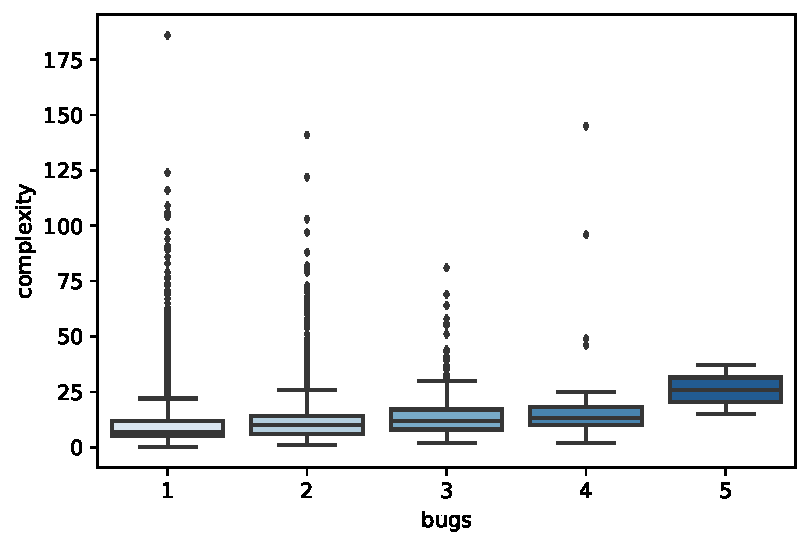
\includegraphics[width=0.7\textwidth]{img/complexity_box.pdf}
    \caption{Number of semantic bugs per query complexity}
    \label{fig:complexity_box}
\end{figure}

\begin{figure}[!htbp]
    \centering
    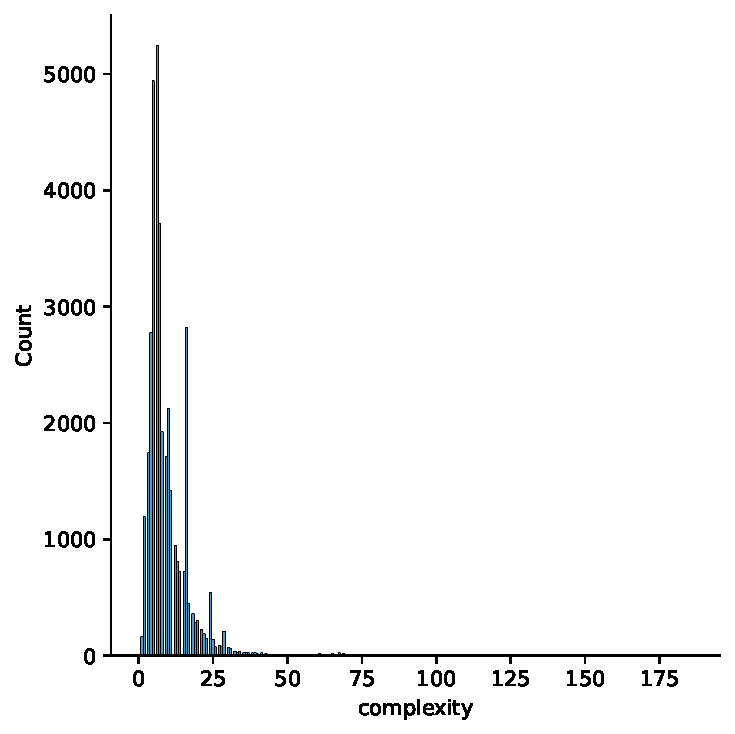
\includegraphics[width=0.7\textwidth]{img/complexity_distribution.pdf}
    \caption{Distribution of query complexity}
    \label{fig:complexity_distribution}
\end{figure}

\newpage
\section{Threats to validity}

In this section, we discuss the threats to the validity of this study and the actions we took to mitigate them.\\

\noindent \textbf{Internal validity.} The implementation of the heuristics for our rule-based static analysis tool can be subject to internal validity threats. To help with overcoming this, each of the 25 rules is covered by an extensive suite of unit tests, for both general as well as special edge case scenarios. Furthermore, we carried out a manual analysis of more than 500 queries, selecting for each of the 25 rules a random subset of 20 queries which were manually checked to ensure the results returned by the heuristics are correct. Finally, we also tried to align, as much as possible, the implementation of our heuristics, with the various implementation details found in previous research.\\

\noindent \textbf{External validity.} Although the collected dataset contains a diverse set of SQL queries, we observed that there are considerably more \sql{SELECT} queries than other types, such as \sql{INSERT}, \sql{UPDATE} or \sql{DELETE} queries, hence these latter types might be underrepresented in this study. This is especially noticeable in the EvoSQL dataset which only contains \sql{SELECT} queries. However, by extracting queries from StackOverflow posts, we hope to have overcome some of these issues, build a diverse enough collection of queries and at the same time have our results generalize on SQL queries in any software system.
